\documentclass[10pt,a4paper]{report}
\usepackage[latin1]{inputenc}
\usepackage{amsmath}
\usepackage{amsfonts}
\usepackage{amssymb}
\usepackage{graphicx}
\usepackage{listings}
\usepackage{multirow}
\lstset{
 	language=Scilab,
 	breaklines = true
 	 }
\title{TRABAJO PR\'ACTICO: HEUR\'ISTICAS Y COTAS INFERIORES PARA EL PROBLEMA DEL VIAJANTE DE COMERCIO (TSP)}
\author{LUCAS SALVATORE}
\date{}
\begin{document}
\maketitle
\begin{enumerate}
\item \underline{Generaci\'on de instancias aleatorias y c\'alculo de valores \'optimos, usando $Concorde$}:\\\\
$\bullet$ Se generaron 10 instancias aleatorias con 100 nodos cada uno. Dichas instancias est\'an en el archivo $instanciaN.tsp$ donde $N$ es el n\'umero de instancia.\\
$\bullet$ Los valores obtenidos por Concorde sobre las instancias aleatorias y las instancias del TSPLIB est\'an en la tabla de la p\'agina $4$.
\item \underline{Comportamiento de la heur\'istica $Vecino$ $mas$ $cercano$}:\\\\
$\bullet$ Se anot\'o, por cada instancia el valor del tour dado por la heur\'istica del Vecino M\'as Cercano. Dichos valores est\'an en la tabla de la p\'agina $4$.
\item \underline{Mejorando la heur\'istica $Vecino$ $mas$ $cercano$}:\\\\
$\bullet$ Se implement\'o la funci\'on \texttt{vecino\_mas\_cercano\_mejorado.sci} que toma una instancia TSP y calcula la heur\'istica del Vecino M\'as Cercano con $v_1 = v$ para cada nodo $v$ del grafo, y devuelve el tour de menor valor. La implementaci\'on se puede ver en el archivo antes mencionado o en las \'ultimas p\'aginas del informe.\\
$\bullet$ La instancia ad-hoc con la que pruebo tanto la heur\'istica del Vecino M\'as Cercano Mejorado como las heur\'isticas siguientes es el grafo $K_4$ con los siguientes costos:
\begin{center}
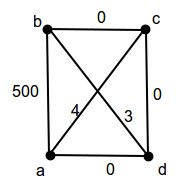
\includegraphics[scale=0.9]{K4.jpg}
\end{center}
$\bullet$ Los valores obtenidos por la heur\'istica sobre las instancias aleatorias y las instancias del TSPLIB junto con el comportamiento promedio est\'an en la tabla de la p\'agina $4$.
\item \underline{Comportamiento de las heur\'isticas de $Insercion$}\\\\
$\bullet$ Se implement\'o la funci\'on \texttt{insercion\_mas\_cercana.sci} que en base a la implementaci\'on de la funci\'on \texttt{insercion\_mas\_lejana.sci}, se modific\'o la iteraci\'on en donde se eleg\'ia el pr\'oximo v\'ertice a insertar en el tour. En la Inserci\'on m\'as Lejana se seleccionaba los v\'ertices con mayor costo. En la Inserci\'on m\'as Cercana se seleccionan los v\'ertices de menor costo. Dicha implementaci\'on se puede ver en el archivo \texttt{.sci} o en las \'ultimas p\'aginas del informe\\
$\bullet$ Los costos de los tours generados por las dos inserciones junto con el promedio, se puede ver en la p\'agina $4$.
\item \underline{Comportamiento de la cota dada por $1$-\'arbol \'optimo}:\\\\
$\bullet$  La implementaci\'on est\'a en el archivo \texttt{uno\_arbol.sci} o se puede ver en la p\'agina $x_4$. La idea del algoritmo es encontrar dos aristas incidentes en el v\'ertice inicial tal que la suma de sus costos sea m\'inima, digamos $a$. Luego buscamos un arbol recubridor m\'inimo del grafo menos el v\'ertice inicial y el costo del arbol lo llamamos $b$. La cota inferior del valor \'optimo del tour ser\'a $a+b$.\\
$\bullet$ Las cotas inferiores dadas por la heur\'isticas del $1$-\'arbol junto con el comportamiento promedio est\'an en la tabla de la p\'agina $4$.
\item \underline{Prueba de las heur\'isticas implementadas}:\\
\begin{lstlisting}[frame=single]
A  =
 
    Inf     0.    500.    3.  
    0.      Inf   4.      0.  
    500.    4.    Inf     0.  
    3.      0.    0.      Inf 
-->[tour,valor] = vecino_mas_cercano(A,1)
 valor  =
 
    500.  
 tour  =
 
    1.  
    2.  
    4.  
    3.
-->[tour,valor] = vecino_mas_cercano_mejor(A)
 valor  =
 
    7.  
 tour  =
 
    2.  
    1.  
    4.  
    3.  
-->[tour,valor] = insercion_mas_cercana(A)
 valor  =
 
    7.  
 tour  =
 
    1.    4.    3.    2.  
-->[tour,valor] = insercion_mas_lejana(A)
 valor  =
 
    7.  
 tour  =
 
    1.    2.    3.    4.
-->uno_arbol(A,1)
 ans  =
 
    3.  
 
-->uno_arbol(A,2)
 ans  =
 
    3.  
 
-->uno_arbol(A,3)
 ans  =
 
    4.  
 
-->uno_arbol(A,4)
 ans  =
 
    4.    
\end{lstlisting}
\end{enumerate}

\newpage
\setcounter{page}{5}
\begin{flushleft}
\underline{Observaciones}:\\
\end{flushleft}
$\bullet$ Se pudo ver que el m\'aximo cociente entre el valor de la heur\'istica del vecino m\'as cercano y el \'optimo se da en la instancia $2$. El gr\'afico siguiente muestra primero el tour \'optimo calculado por Concorde y luego se muestra el tour calculado por la heur\'istica. \\
\begin{center}
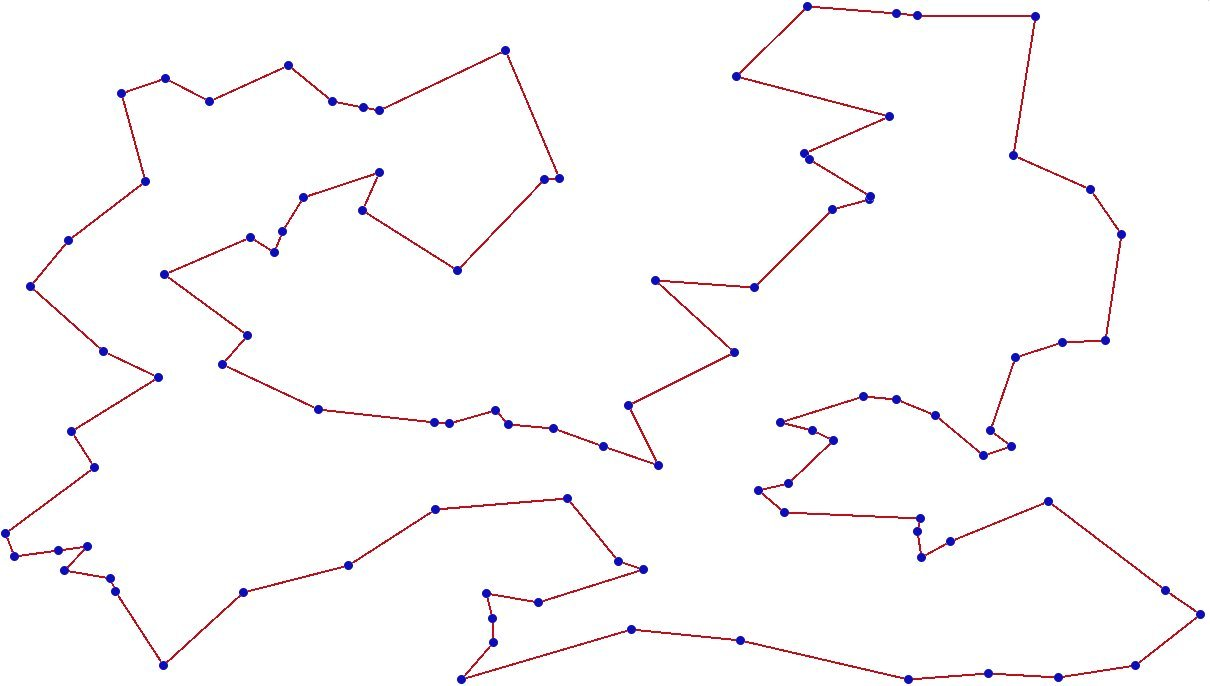
\includegraphics[scale=0.3]{instancia2TourOpt.jpg}
\end{center}
\begin{center}
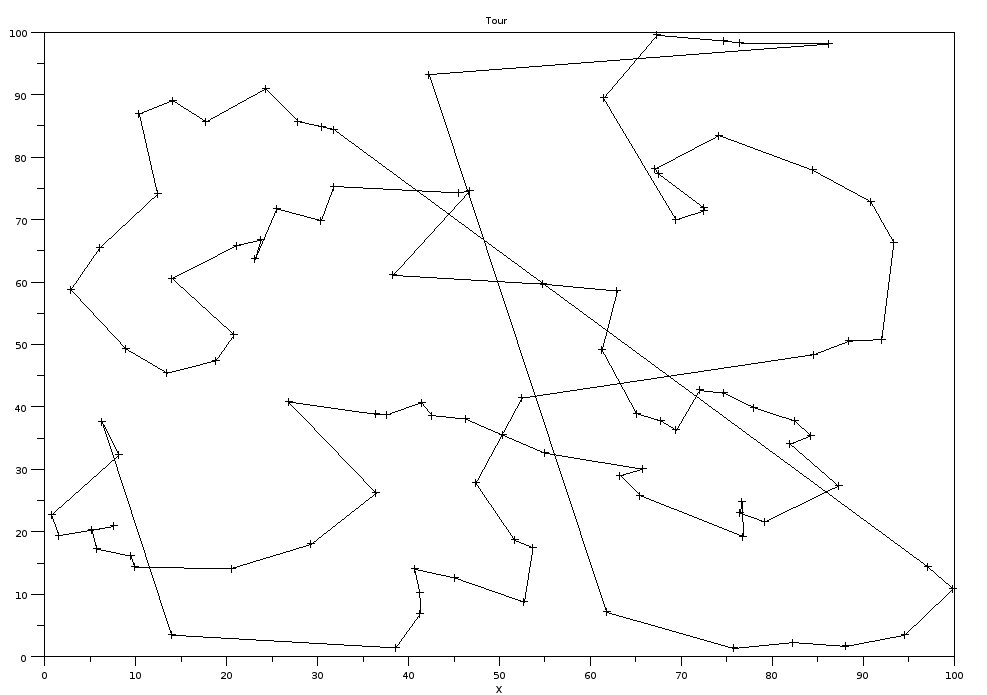
\includegraphics[scale=0.4]{instancia2TourVMC.jpg}
\end{center}
\ \\\\\\\\
$\bullet$ De acuerdo a los valores promedios provistos por la tabla y los valores promedios brindados por el libro de Cook, se puede ver que no var\'ia tanto los valores, siendo la m\'axima diferencia de $0.06$ para la heur\'istica de la inserci\'on m\'as lejana:
\begin{table}[htbp]
\begin{center}
\begin{tabular}{|l|l|l|}
\hline
Heuristica & Tabla & Libro Cook\\
\hline
Vecino M\'as Cercano & $1.24\times OPT$ & $1.26\times OPT$\\
Insercion M\'as Lejana & $1.10\times OPT$ & $1.16\times OPT$\\
Cota $1$-\'arbol & $0.88\times OPT$ & $0.90 \times OPT$\\ 
\hline
\end{tabular}
\end{center}
\end{table}
\\
$\bullet$ Viendo el cuadro y en base a los valores reportados por las 20 instancias TSP, se puede apreciar que la heur\'istica que m\'as se acerca al valor o\'ptimo es la inserci\'on m\'as lejana. Tal como dice Cook en el libro, se puede deber a que en las primeras etapas de la construcci\'on del tour, ya se nota la forma que tomar\'a, y en las \'ultimas etapas las modificaciones ya son m\'as leves.
\begin{flushleft}
\underline{Implementaciones}:\\
\end{flushleft}
En las siguientes 3 hojas se muestran las implementaciones de los c\'odigos del vecino m\'as cercano mejorado, la inserci\'on m\'as cercana y el algoritmo del $1$-arbol para determinar la cota inferior.
\end{document}